% GNUPLOT: LaTeX picture with Postscript
\begingroup
  \makeatletter
  \providecommand\color[2][]{%
    \GenericError{(gnuplot) \space\space\space\@spaces}{%
      Package color not loaded in conjunction with
      terminal option `colourtext'%
    }{See the gnuplot documentation for explanation.%
    }{Either use 'blacktext' in gnuplot or load the package
      color.sty in LaTeX.}%
    \renewcommand\color[2][]{}%
  }%
  \providecommand\includegraphics[2][]{%
    \GenericError{(gnuplot) \space\space\space\@spaces}{%
      Package graphicx or graphics not loaded%
    }{See the gnuplot documentation for explanation.%
    }{The gnuplot epslatex terminal needs graphicx.sty or graphics.sty.}%
    \renewcommand\includegraphics[2][]{}%
  }%
  \providecommand\rotatebox[2]{#2}%
  \@ifundefined{ifGPcolor}{%
    \newif\ifGPcolor
    \GPcolortrue
  }{}%
  \@ifundefined{ifGPblacktext}{%
    \newif\ifGPblacktext
    \GPblacktexttrue
  }{}%
  % define a \g@addto@macro without @ in the name:
  \let\gplgaddtomacro\g@addto@macro
  % define empty templates for all commands taking text:
  \gdef\gplbacktext{}%
  \gdef\gplfronttext{}%
  \makeatother
  \ifGPblacktext
    % no textcolor at all
    \def\colorrgb#1{}%
    \def\colorgray#1{}%
  \else
    % gray or color?
    \ifGPcolor
      \def\colorrgb#1{\color[rgb]{#1}}%
      \def\colorgray#1{\color[gray]{#1}}%
      \expandafter\def\csname LTw\endcsname{\color{white}}%
      \expandafter\def\csname LTb\endcsname{\color{black}}%
      \expandafter\def\csname LTa\endcsname{\color{black}}%
      \expandafter\def\csname LT0\endcsname{\color[rgb]{1,0,0}}%
      \expandafter\def\csname LT1\endcsname{\color[rgb]{0,1,0}}%
      \expandafter\def\csname LT2\endcsname{\color[rgb]{0,0,1}}%
      \expandafter\def\csname LT3\endcsname{\color[rgb]{1,0,1}}%
      \expandafter\def\csname LT4\endcsname{\color[rgb]{0,1,1}}%
      \expandafter\def\csname LT5\endcsname{\color[rgb]{1,1,0}}%
      \expandafter\def\csname LT6\endcsname{\color[rgb]{0,0,0}}%
      \expandafter\def\csname LT7\endcsname{\color[rgb]{1,0.3,0}}%
      \expandafter\def\csname LT8\endcsname{\color[rgb]{0.5,0.5,0.5}}%
    \else
      % gray
      \def\colorrgb#1{\color{black}}%
      \def\colorgray#1{\color[gray]{#1}}%
      \expandafter\def\csname LTw\endcsname{\color{white}}%
      \expandafter\def\csname LTb\endcsname{\color{black}}%
      \expandafter\def\csname LTa\endcsname{\color{black}}%
      \expandafter\def\csname LT0\endcsname{\color{black}}%
      \expandafter\def\csname LT1\endcsname{\color{black}}%
      \expandafter\def\csname LT2\endcsname{\color{black}}%
      \expandafter\def\csname LT3\endcsname{\color{black}}%
      \expandafter\def\csname LT4\endcsname{\color{black}}%
      \expandafter\def\csname LT5\endcsname{\color{black}}%
      \expandafter\def\csname LT6\endcsname{\color{black}}%
      \expandafter\def\csname LT7\endcsname{\color{black}}%
      \expandafter\def\csname LT8\endcsname{\color{black}}%
    \fi
  \fi
    \setlength{\unitlength}{0.0500bp}%
    \ifx\gptboxheight\undefined%
      \newlength{\gptboxheight}%
      \newlength{\gptboxwidth}%
      \newsavebox{\gptboxtext}%
    \fi%
    \setlength{\fboxrule}{0.5pt}%
    \setlength{\fboxsep}{1pt}%
\begin{picture}(9340.00,5660.00)%
    \gplgaddtomacro\gplbacktext{%
      \colorrgb{0.00,0.00,0.00}%%
      \put(655,787){\makebox(0,0)[r]{\strut{} 0}}%
      \colorrgb{0.00,0.00,0.00}%%
      \put(655,1304){\makebox(0,0)[r]{\strut{} 10}}%
      \colorrgb{0.00,0.00,0.00}%%
      \put(655,1821){\makebox(0,0)[r]{\strut{} 20}}%
      \colorrgb{0.00,0.00,0.00}%%
      \put(655,2338){\makebox(0,0)[r]{\strut{} 30}}%
      \colorrgb{0.00,0.00,0.00}%%
      \put(655,2855){\makebox(0,0)[r]{\strut{} 40}}%
      \colorrgb{0.00,0.00,0.00}%%
      \put(655,3372){\makebox(0,0)[r]{\strut{} 50}}%
      \colorrgb{0.00,0.00,0.00}%%
      \put(655,3889){\makebox(0,0)[r]{\strut{} 60}}%
      \colorrgb{0.00,0.00,0.00}%%
      \put(655,4406){\makebox(0,0)[r]{\strut{} 70}}%
      \colorrgb{0.00,0.00,0.00}%%
      \put(655,4923){\makebox(0,0)[r]{\strut{} 80}}%
      \colorrgb{0.00,0.00,0.00}%%
      \put(655,5440){\makebox(0,0)[r]{\strut{} 90}}%
      \colorrgb{0.00,0.00,0.00}%%
      \put(839,481){\makebox(0,0){\strut{} 1200}}%
      \colorrgb{0.00,0.00,0.00}%%
      \put(2075,481){\makebox(0,0){\strut{} 1250}}%
      \colorrgb{0.00,0.00,0.00}%%
      \put(3312,481){\makebox(0,0){\strut{} 1300}}%
      \colorrgb{0.00,0.00,0.00}%%
      \put(4548,481){\makebox(0,0){\strut{} 1350}}%
      \colorrgb{0.00,0.00,0.00}%%
      \put(5784,481){\makebox(0,0){\strut{} 1400}}%
      \colorrgb{0.00,0.00,0.00}%%
      \put(7021,481){\makebox(0,0){\strut{} 1450}}%
      \colorrgb{0.00,0.00,0.00}%%
      \put(8257,481){\makebox(0,0){\strut{} 1500}}%
      \colorrgb{0.00,0.00,0.00}%%
      \put(8441,787){\makebox(0,0)[l]{\strut{} 0}}%
      \colorrgb{0.00,0.00,0.00}%%
      \put(8441,1304){\makebox(0,0)[l]{\strut{} 5}}%
      \colorrgb{0.00,0.00,0.00}%%
      \put(8441,1821){\makebox(0,0)[l]{\strut{} 10}}%
      \colorrgb{0.00,0.00,0.00}%%
      \put(8441,2338){\makebox(0,0)[l]{\strut{} 15}}%
      \colorrgb{0.00,0.00,0.00}%%
      \put(8441,2855){\makebox(0,0)[l]{\strut{} 20}}%
      \colorrgb{0.00,0.00,0.00}%%
      \put(8441,3372){\makebox(0,0)[l]{\strut{} 25}}%
      \colorrgb{0.00,0.00,0.00}%%
      \put(8441,3889){\makebox(0,0)[l]{\strut{} 30}}%
      \colorrgb{0.00,0.00,0.00}%%
      \put(8441,4406){\makebox(0,0)[l]{\strut{} 35}}%
      \colorrgb{0.00,0.00,0.00}%%
      \put(8441,4923){\makebox(0,0)[l]{\strut{} 40}}%
      \colorrgb{0.00,0.00,0.00}%%
      \put(8441,5440){\makebox(0,0)[l]{\strut{} 45}}%
    }%
    \gplgaddtomacro\gplfronttext{%
      \csname LTb\endcsname%%
      \put(255,3113){\rotatebox{-270}{\makebox(0,0){\strut{}$T\ped{m}\, / \,\si{N.m}, \quad T\ped{load}\, / \,\si{N.m}$}}}%
      \csname LTb\endcsname%%
      \put(8938,3113){\rotatebox{-270}{\makebox(0,0){\strut{}$I_1\, / \,\si{A}$}}}%
      \csname LTb\endcsname%%
      \put(4548,153){\makebox(0,0){\strut{}$n\ped{m}\, / \,\si{r/min}$}}%
      \csname LTb\endcsname%%
      \put(4548,5331){\makebox(0,0){\strut{}}}%
      \csname LTb\endcsname%%
      \put(4548,5440){\makebox(0,0){\strut{}}}%
      \csname LTb\endcsname%%
      \put(1513,2079){\makebox(0,0){\strut{}}}%
      \csname LTb\endcsname%%
      \put(1314,1969){\makebox(0,0)[l]{\strut{}$T\ped{load}$}}%
      \csname LTb\endcsname%%
      \put(1314,1750){\makebox(0,0)[l]{\strut{}$T\ped{m,\SI{100}{\%}}$}}%
      \csname LTb\endcsname%%
      \put(1314,1531){\makebox(0,0)[l]{\strut{}$T\ped{m,\SI{80}{\%}}$}}%
      \csname LTb\endcsname%%
      \put(1314,1312){\makebox(0,0)[l]{\strut{}$I\ped{1,\SI{100}{\%}}$}}%
      \csname LTb\endcsname%%
      \put(1314,1093){\makebox(0,0)[l]{\strut{}$I\ped{1,\SI{80}{\%}}$}}%
      \csname LTb\endcsname%%
      \put(6452,1563){\rotatebox{-270}{\makebox(0,0){$\scriptstyle\SI{1431}{r/min}$}}}%
      \csname LTb\endcsname%%
      \put(5381,1563){\rotatebox{-270}{\makebox(0,0){$\scriptstyle\SI{1387,5}{r/min}$}}}%
      \csname LTb\endcsname%%
      \put(1581,3786){\makebox(0,0){$\scriptstyle\SI{56,6}{N.m}$}}%
      \csname LTb\endcsname%%
      \put(1581,3450){\makebox(0,0){$\scriptstyle\SI{53,4}{N.m}$}}%
      \csname LTb\endcsname%%
      \put(7762,2576){\makebox(0,0){$\scriptstyle\SI{16,6}{A}$}}%
      \csname LTb\endcsname%%
      \put(7762,2917){\makebox(0,0){$\scriptstyle\SI{19,6}{A}$}}%
    }%
    \gplbacktext
    \put(0,0){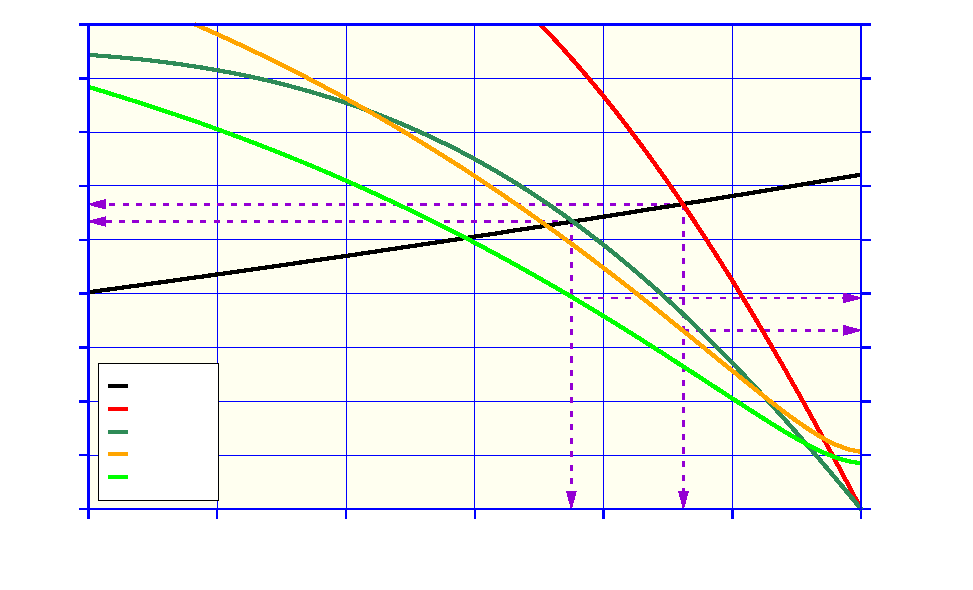
\includegraphics{Cap-Motors-Induccio-Ex8-1-2}}%
    \gplfronttext
  \end{picture}%
\endgroup
